\documentclass[10pt]{beamer}

\usetheme{default}

\usepackage[utf8]{inputenc}
\usepackage[russian]{babel}
\usepackage[OT1]{fontenc}
\usepackage{amsmath}
\usepackage{amsfonts}
\usepackage{amssymb}
\usepackage{graphicx}
\usepackage{etoolbox}
\usepackage{caption}
\usepackage{subcaption}
\captionsetup{compatibility=false}
\usepackage{booktabs}
\usepackage{array}



\makeatletter



\setbeamercolor{title}{fg=white}
\setbeamercolor{frametitle}{fg=black}
\setbeamerfont*{title}{family=\sffamily,size=\LARGE}

\setbeamerfont{page number in head/foot}{size=\scriptsize}
\setbeamertemplate{footline}[frame number]
\let\otp\titlepage
\renewcommand{\titlepage}{\otp\addtocounter{framenumber}{-1}}

\setbeamertemplate{background canvas}{%
	\ifnumequal{\c@framenumber}{0}{%
      
\includegraphics[width=\paperwidth,height=\paperheight]{images/cover.png}
   }{%
      \ifnumequal{\c@framenumber}{\inserttotalframenumber}{
         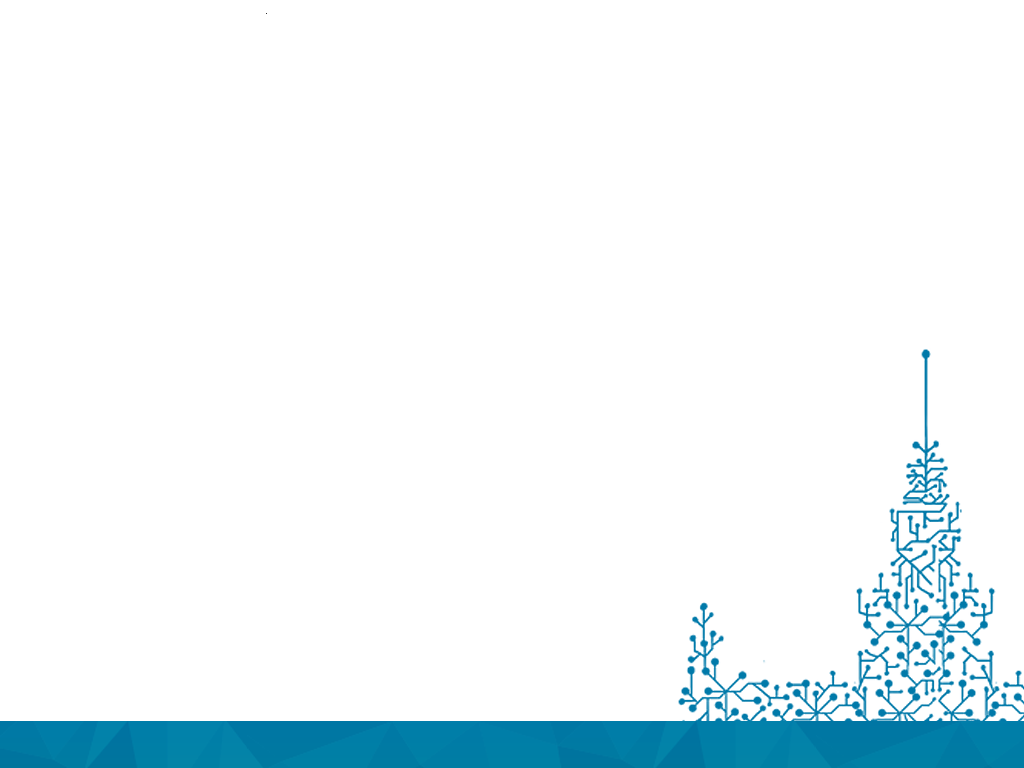
\includegraphics[width=\paperwidth,height=\paperheight]{images/back.png}
      }{%
         % Other frames
      }%
   }%
}

\makeatother

\beamertemplatenavigationsymbolsempty

\author{Нестеров Павел}
\title{\newline \newline \newline Лекция n1 \\ Основы нейронных сетей}

\begin{document}

\begin{frame}[plain]
\titlepage
\end{frame}

\begin{frame}{План лекции}
\tableofcontents
\end{frame}


\section{Предпосылки}

\begin{frame}{Принципиальное отличие}

\begin{description}
  \item[Теория статистического обучения] \hfill \\
  Линейная и логистическая регрессии, expectation-maximization, naive bayes classifier, random forest, support vectior machine, gradient boosting trees и т.д.
  \item[Имитация работы мозга человека] \hfill \\
  Perceptron, cognitron, self-organizing maps, multi-layer feedforward network, convolution network, Boltzmann machine, deep neural network и т.д. \\
\end{description}

\end{frame}


\begin{frame}{С другой стороны}

\begin{block}{Искусственная нейронная сеть}
\begin{itemize}
  \item алгоритмическая композиция (ансамбль) слабых моделей
  \item байесова или марковская сеть
  \item ???
  \item или любое другое \textit{обобщение}, важны идеи лежащие в основе теории
\end{itemize}
\end{block}

\end{frame}


\begin{frame}{Нервная система до нейробиологии}

\begin{figure}[h!]
  \centering
  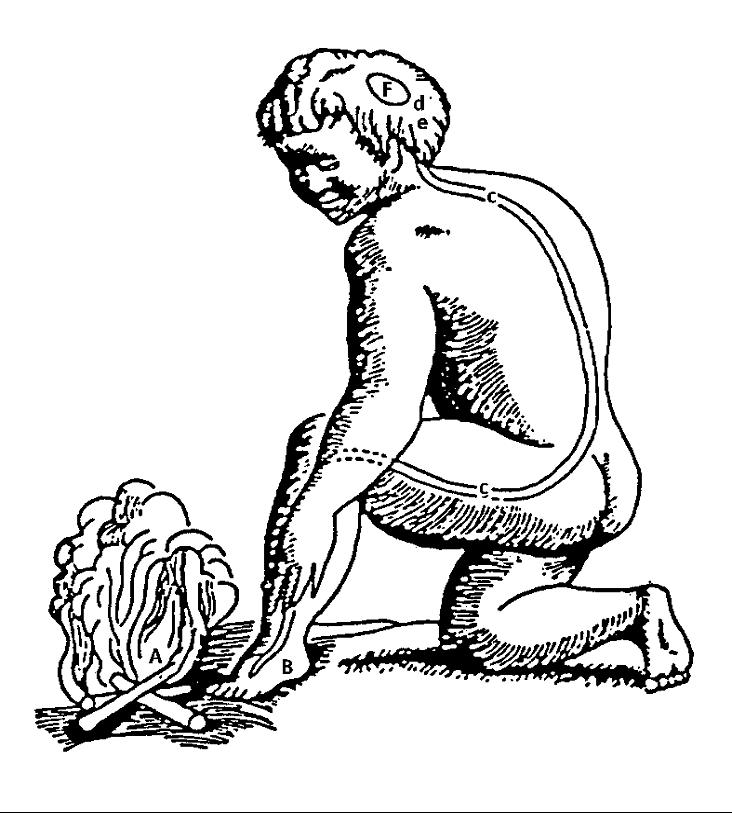
\includegraphics[width=0.5\textwidth]{images/Reizweiterleitung.jpg}
  \caption{17 век, Рене Декарт о нервной системе: «Раздражение ступни передаётся по нервам в мозг, взаимодействует там с духом и таким образом порождает ощущение боли».}
\end{figure}

\end{frame}


\begin{frame}{Нервная система в современном понимании}

\begin{itemize}
	\item В 1906 году врач и гистолог Сантьяго Рамон-и-Кахаль совместно с врачем Камилло Гольджи получают нобелевскую премию за "за работы по структуре нервной системы"; их работы заложили основы нейронной теории нервной системы и современной нейробиологии.
\end{itemize}

\begin{figure}[h!]
  \centering
  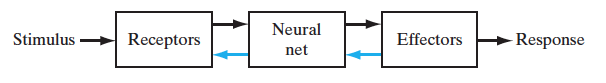
\includegraphics[width=1\textwidth]{images/bd_nervous_system.png}
  \caption{Блок-схема нервной системы\footnote{Neural Networks and Learning Machines (3rd Edition), Simon O. Haykin}}
\end{figure}

\end{frame}


\begin{frame}{Мозг человека, \#1}

\begin{figure}[h!]
  \centering
  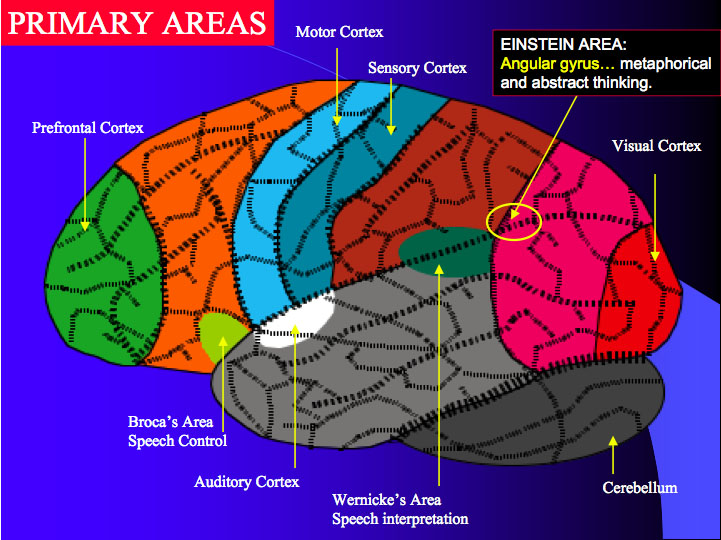
\includegraphics[width=1\textwidth]{images/Brain_2.jpg}
\end{figure}

\end{frame}


\begin{frame}{Мозг человека, \#2}

\begin{columns}
    \column{0.3\textwidth}
    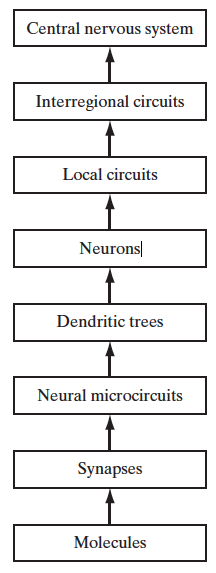
\includegraphics[width=1\textwidth]{images/bd_brain.png}
    \column{0.7\textwidth}
	\begin{itemize}
		\item $86\cdot10^9$ нейронов в мозге, из них $16.3\cdot10^9$ в коре
		\begin{itemize}
			\item CPU: \textit{15-core Xeon IvyBridge-EX} - $4.3\cdot10^9$ транзисторов
			\item GPU: \textit{Nvidia Tesla GK110 Kepler} - $7.08\cdot10^9$ транзисторов
		\end{itemize}
		\item нейроны (и мозг в целом) обладают \textbf{нейропластичностью} - способностью изменяться под действием опыта;
		\item мозг - комплексная, нелинейная система параллельной обработки данных, способная изменять структуру своих составных частей;
		\item мозг решает определенный тип задач значительно быстрее чем любой современный компьютер, несмотря на то, что нейрон крайне \textit{медленная} вычислительная единица.
	\end{itemize}	    
\end{columns}

\end{frame}


\begin{frame}{Схема биологического нейрона}

\centering
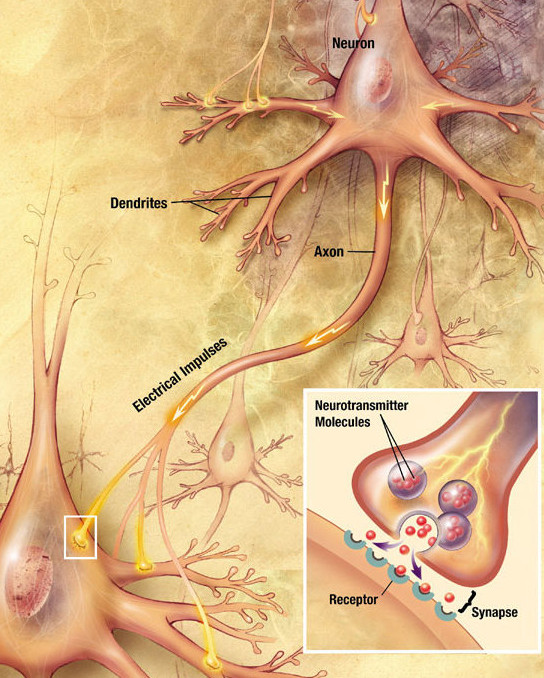
\includegraphics[width=0.63\textwidth]{images/Chemical_synapse_schema_cropped.jpg}

\end{frame}


\begin{frame}{Нейронные ансамбли}

\begin{itemize}
	\item Физиолог и нейропсихолог Дональд Хебб разработал теорию взаимосвязи головного мозга и мыслительных процессов в книге "The Organization of Behavior" (1949).
	\item Нейронный ансамбль - совокупность нейронов, составляющих функциональную группу в высших отделах мозга.
	\item Нейроансамбль - распределенный способ кодирования информации.
	\item Нейрон сам по себе генерирует по мимо сигнала еще и шум, но ансамбль в среднем генерирует чистый сигнал (\textit{bagging?}).
\end{itemize}


\end{frame}


\begin{frame}{Нейронная модель Ходжкина-Хаксли, \#1}

\begin{itemize}
	\item Модель Ходжкина—Хаксли (1952 год) — математическая модель, описывающая генерацию и распространение потенциалов действия в нейронах\footnote{см. приложение Cellmembranion.gif}.
	\item Потенциал действия — волна возбуждения, перемещающаяся по мембране живой клетки в процессе передачи нервного сигнала.
	\item Нобелевская премия по физиологии и медицине "за открытия, касающиеся ионных механизмов возбуждения и торможения в периферических и центральных участках нервных клеток" (1963 год). 
\end{itemize}


\end{frame}


\begin{frame}{Нейронная модель Ходжкина-Хаксли, \#2}

\centering
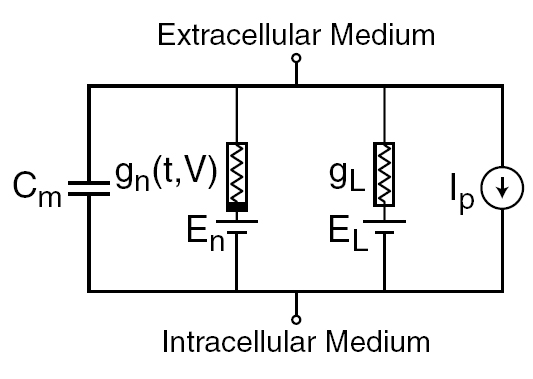
\includegraphics[width=0.5\textwidth]{images/Hodgkin-Huxley.jpg}\\
Каждому элементу схемы соответствует свой биохимический аналог:
\begin{itemize}
	\item $C_m$ - электроемкость внутреннего липидного слоя клеточной мембраны;
	\item $g_n$ - потенциал-зависимые ионные каналы отвечают за нелинейную электрическую проводимость;
	\item $g_L$ - каналы мембранных пор отвечают за пассивную проводимость;
	\item $E_x$ - источники напряжения побуждает ионы к движению через мембранные каналы.
\end{itemize}


\end{frame}


\section{Краткая история теории нейронных сетей}

\begin{frame}{Модель МакКаллока-Питтса (1943 год)}

\centering
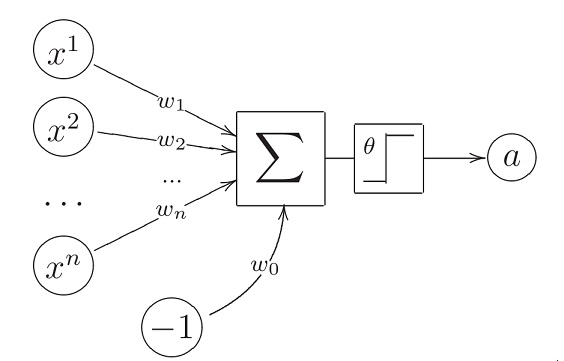
\includegraphics[width=0.7\textwidth]{images/neuron_m_p.jpg}
\begin{itemize}
	\item $a\left(x\right) = \theta\left(\sum_{j = 1}^{n}w_j \cdot x_i - w_0\right)$;
	\item $\theta\left(z\right) = \left[z \geq 0 \right] = \left\{ {0, z < 0\atop1, z \geq 0} \right.$ - функция Хевисайда;
	\item эквивалентно линейному классификатору.
\end{itemize}
\begin{flushleft}
Данная модель, с незначительными изменениями, актуальна и по сей день.
\end{flushleft}

\end{frame}


\begin{frame}{Правила Хебба (1949)}
В своей книге Дональд Хебб описал процесс адаптирования нейронов в мозге в процессе обучения, и сформулировал базовые механизмы нейропластичности:
\begin{enumerate}
	\item если два нейрона по разные стороны от синапсов активируются синхронно, то "вес" синапса слегка возрастает;
	\item если два нейрона по разные стороны от синапсов активируются асинхронно, то "вес" синапса слегка ослабевает или синапс удаляется\footnote{это расширенное правило, в оригинале второй части не было}.
\end{enumerate}
Эти правила легли в основу зарождающейся теории нейросетей, сегодня в мы можем увидеть этот мета-алгоритм в основных методах обучения нейронных сетей.

\end{frame}


\begin{frame}{Правила Хебба, математическая формулировка, \#1}

Допустим у нас имеется набор бинарных векторов размерности $n$, каждому из которых соответствует бинарный выход $y$:
\begin{itemize}
	\item $X = \left\{\vec x_1, \vec x_2, \ldots, \vec x_m\right\}, \forall \vec x_i \in \left\{0, 1\right\}^n$
	\item $Y = \left\{y_1, y_2, \ldots, y_m\right\}, \forall y_i \in \left\{0, 1\right\}$
	\item $D = \left\{ \left(x_1, y_1\right), \left(x_2, y_2\right), \ldots, \left(x_n, y_n\right) \right\}$
\end{itemize}
Тогда нейрон может совершить два типа ошибок:
\begin{enumerate}
	\item $\hat y_i = 0 \wedge y_i = 1 \Rightarrow $ \textit{увеличить} веса при тех входах равных 1
	\begin{itemize}
		\item \textit{зачем?}
	\end{itemize}
	\item $\hat y_i = 1 \wedge y_i = 0 \Rightarrow $ \textit{уменьшить} веса при тех входах равных 1
	\begin{itemize}
		\item \textit{зачем?}
	\end{itemize}
\end{enumerate}


\end{frame}


\begin{frame}{Правила Хебба, математическая формулировка, \#2}

Тогда нейрон может совершить два типа ошибок:
\begin{enumerate}
	\item $\hat y_i = 0 \wedge y_i = 1 \Rightarrow $ \textit{увеличить} веса при тех входах равных 1
	\begin{itemize}
		\item не преодолели порог $\Rightarrow$ увеличить скалярное произведение
	\end{itemize}
	\item $\hat y_i = 1 \wedge y_i = 0 \Rightarrow $ \textit{уменьшить} веса при тех входах равных 1
	\begin{itemize}
		\item перешагнули порог $\Rightarrow$ уменьшить скалярное произведение
	\end{itemize}
\end{enumerate}
\centering
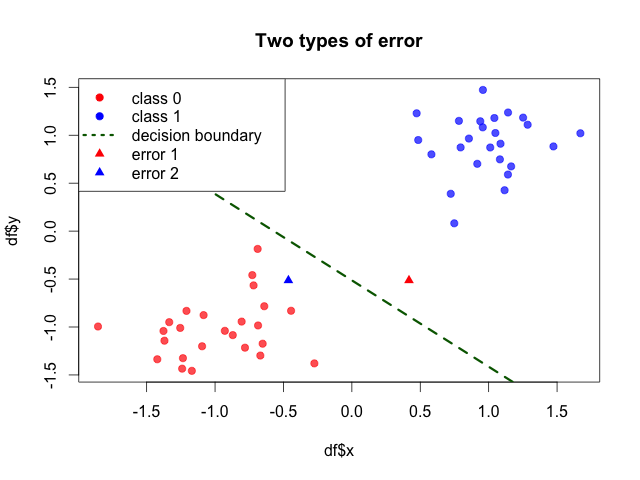
\includegraphics[width=0.8\textwidth]{images/two_types_errors.png}

\end{frame}


\begin{frame}{Однослойный персептрон Розенблатта (1958 год)}

Нейрофизиолог Френк Розенблатт предложил схему устройства, моделирующего процесс человеческого восприятия, и назвал его "персептроном". По мимо этого:
\begin{itemize}
	\item показал, что персептрон может выполнять базовые логические операции;
	\item разработал алгоритм обучения такой модели - метод коррекции ошибки;
	\item доказал сходимость алгоритма (теорема сходимости персептрона), но только для линейно разделимых классов;
	\item реализовал физический прототип такой модели;
	\item реализовал первый в мире нейрокомпьютер "MARK-1".
\end{itemize}

\end{frame}


\begin{frame}{Нейрокомпьютер MARK-1}

\begin{figure}
        \centering
        \begin{subfigure}[b]{0.4\textwidth}
                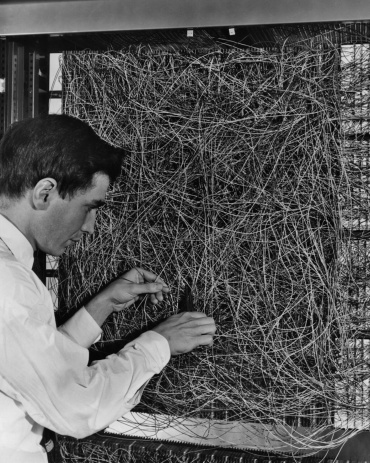
\includegraphics[width=\textwidth]{images/rosenblatt1.jpg}
        \end{subfigure}%        
        \begin{subfigure}[b]{0.5\textwidth}
                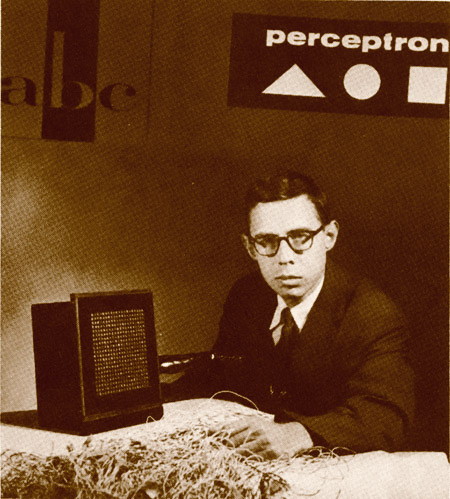
\includegraphics[width=0.9\textwidth]{images/rosenblatt2.jpg}
        \end{subfigure}
\end{figure}

\end{frame}


\begin{frame}{Элементарный персептрон}

\centering
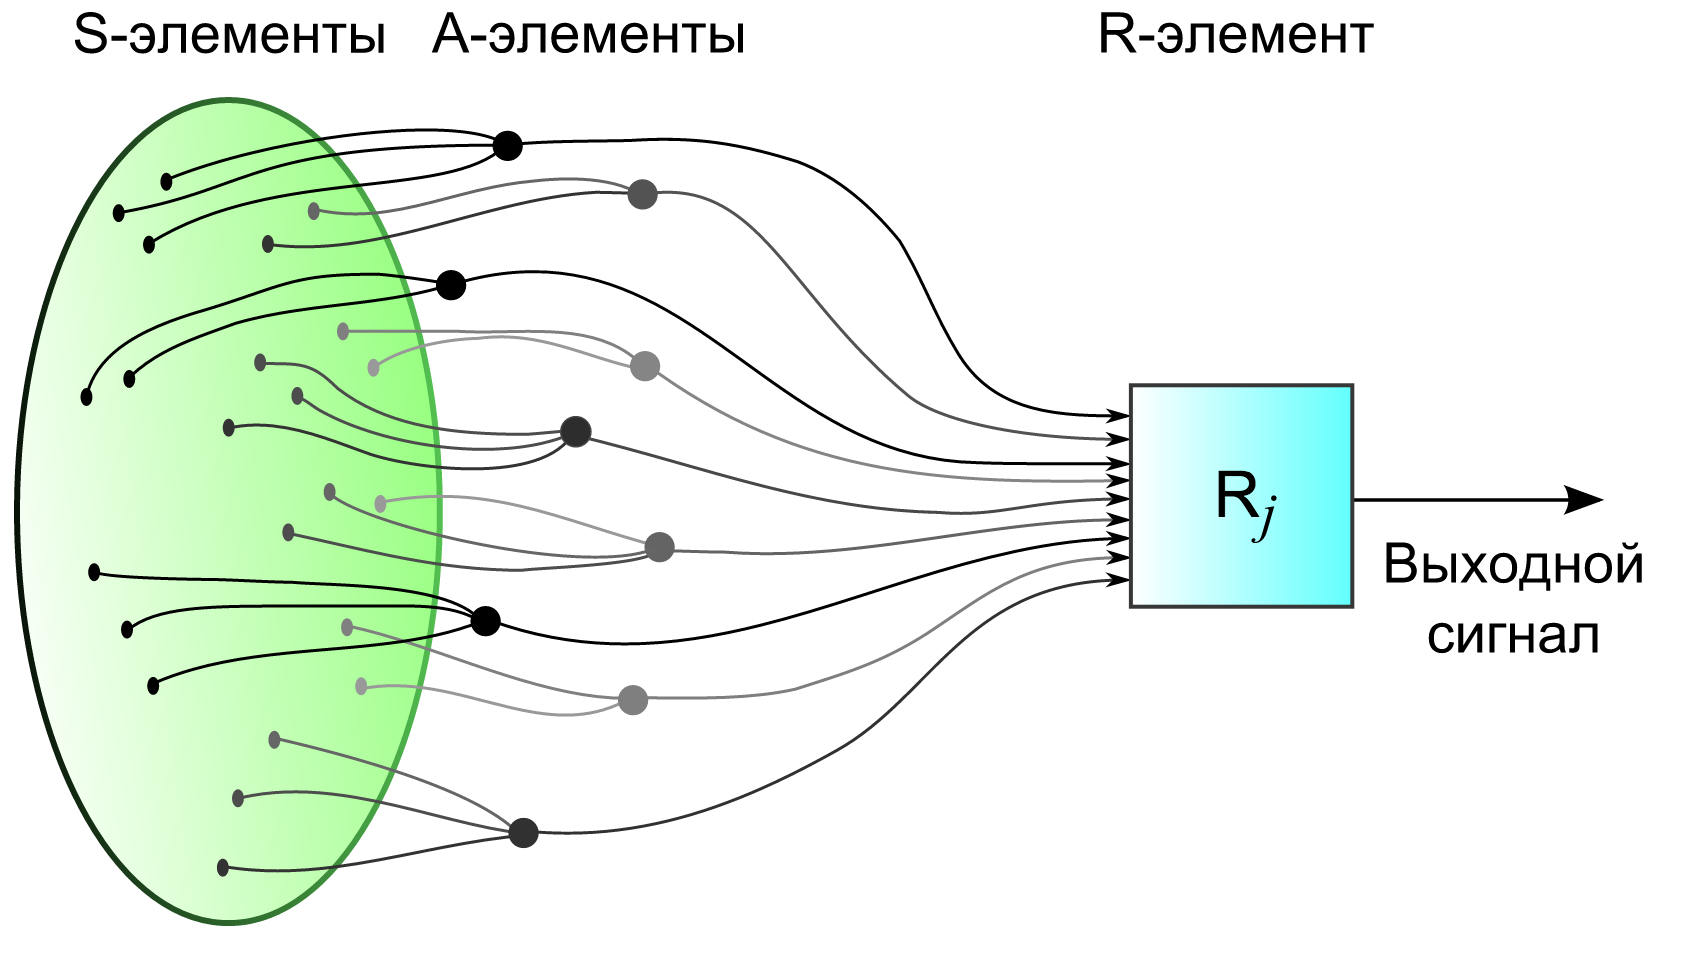
\includegraphics[width=0.7\textwidth]{images/perceptron.png}
\begin{flushleft}
Метод коррекции ошибки
\begin{itemize}
	\item $\hat y_i = 0 \wedge y_i = 1 \Rightarrow \Delta w = \eta(n)\cdot x(n)$
	\item $\hat y_i = 1 \wedge y_i = 0 \Rightarrow \Delta w = -\eta(n)\cdot x(n)$
	\begin{itemize}
		\item $\eta(n)$ - скорость обучения, зависящая от итерации
		\item $x(n)$ - входной образ на итерации $n$
	\end{itemize}
\end{itemize}
\end{flushleft}

\end{frame}


\begin{frame}{Недостатки элементарного персептрона, AND}

\centering
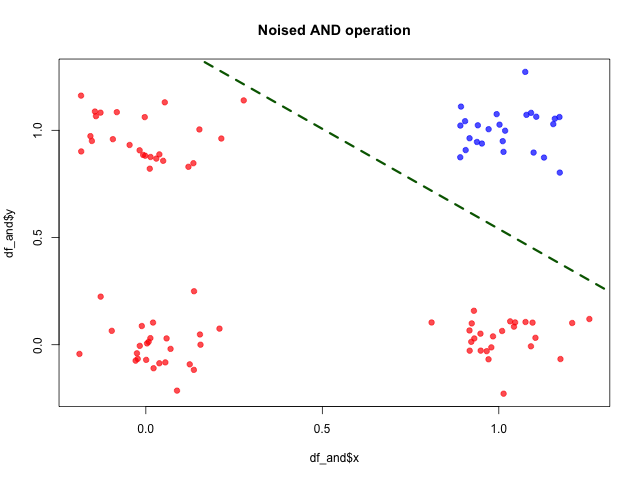
\includegraphics[width=1\textwidth]{images/leakage_perceptron_and.png}

\end{frame}


\begin{frame}{Недостатки элементарного персептрона, XOR}

\centering
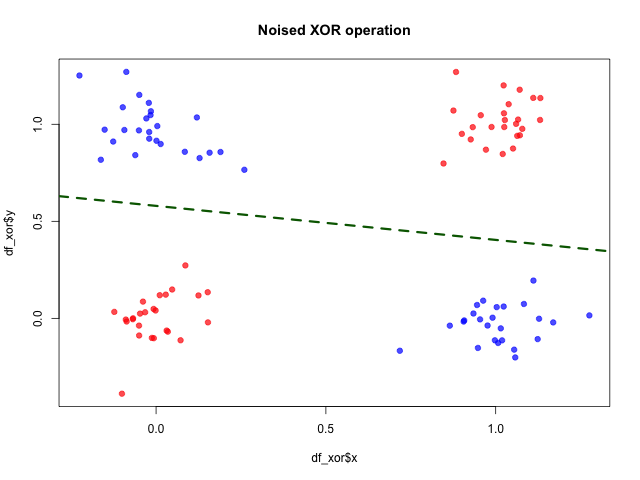
\includegraphics[width=1\textwidth]{images/leakage_perceptron_xor.png}

\end{frame}


\begin{frame}{Анимация сходимости для операций AND и XOR}

\begin{itemize}
	\item операция OR  - 1layer-net-or.gif
	\item операция AND - 1layer-net-and1.gif
	\item операция XOR - 1layer-net-xor.gif \footnote{http://theclevermachine.wordpress.com/2014/09/11/a-gentle-introduction-to-artificial-neural-networks/}
\end{itemize}

\end{frame}


\begin{frame}{Доказательства неэффективности нейронных сетей}

\begin{itemize}
	\item В 1969 году математик и исследователь ИИ Марвин Минский провел детальный математический анализ  персептрона и опубликовал формальное доказательство ограниченности этой модели.
	\item \textit{"\textbf{There is no reason to suppose} that any of these virtues carry over to the many-layered version. Nevertheless, we consider it to be an important research problem to elucidate (or reject) our intuitive judgement that the extension to multilayer systems is sterile."}\footnote{Персептроны, Марвин Минский в соавторстве с Сеймуром Папертом, MIT Press, 1969}
	\item Отсутствие преимуществ + ограничения модели в итоге поубавили интерес научного сообщества к нейронным сетям, требовалось, что то принципиально новое
\end{itemize}

\end{frame}


\begin{frame}{Период "забвения"}

Исследования \textit{искусственных} нейросетей не спеша продолжаются, но в режиме поиска чего-то нового:
\begin{itemize}
	\item 1972: Т. Кохонен разрабатывает новый тип нейросетей, способных функционировать в качестве памяти;
	\item 1975-1980: К. Фукусима разрабатывает когнитрон и неокогнитрон, совершенно новый тип многослойной сверточной сети, созданной по аналогии со строением зрительной системы;
	\item 1982: Дж. Хопфилд разрабатывает новый тип нейросети с обратными связями, выполняющей функции ассоциативной памяти;
	\item 1986: Дэвид Румельхарт, \textbf{Дж. Хинтон} и Рональд Вильямс разрабатывают \textit{вычислительно эффективный} многослойных нейросетей - метод обратного распространения ошибки (именно работа этих авторов возрождает интерес к нейронным сетям в мире).
\end{itemize}

\end{frame}


\section{Многоснойная нейронная сеть прямого распространения}

\begin{frame}{Теорема универсальной аппроксимации\footnote{Neural Networks and Learning Machines (3rd Edition), Simon O. Haykin}}

Введем следующие обозначения:
\begin{itemize}
	\item $\phi(x)$ - не тождественная, ограниченная и монотонно возрастающая функция
	\item $I_{n}$ - $n$-мерный единичный гиперкуб
	\item $C\left(I_{n}\right)$ - множество непрерывных функций на $I_{n}$
\end{itemize}
$\Rightarrow \forall f \wedge \forall \epsilon > 0 \exists$
\begin{itemize}
	\item $m \in \mathbb{N}$
	\item $\left\{\beta_i\right\}_{i=1\ldots m}, \forall \beta_i \in \mathbb{R}$
	\item $\left\{\alpha_i\right\}_{i=1\ldots m}, \forall \alpha_i \in \mathbb{R}$
	\item $\left\{w_{ij}\right\}_{j=1\ldots n, i=1\ldots m}, \forall w_{ij} \in \mathbb{R}$
\end{itemize}
$\wedge \exists F\left(x_1, \ldots, x_n\right) = \sum_{i=1}^m \alpha_i \phi \left( \sum_{j=1}^n w_{ij}\cdot x_j + \beta_i \right):$
\begin{itemize}
	\item $\left| F\left(x_1, \ldots, x_n\right) - f\left(x_1, \ldots, x_n\right) \right| < \epsilon$
\end{itemize}
\textit{Какая архитектура нейросети удовлетворяет такой формулировке?}
\end{frame}

\begin{frame}{Универсальный аппроксиматор}

\begin{figure}[h!]
\centering
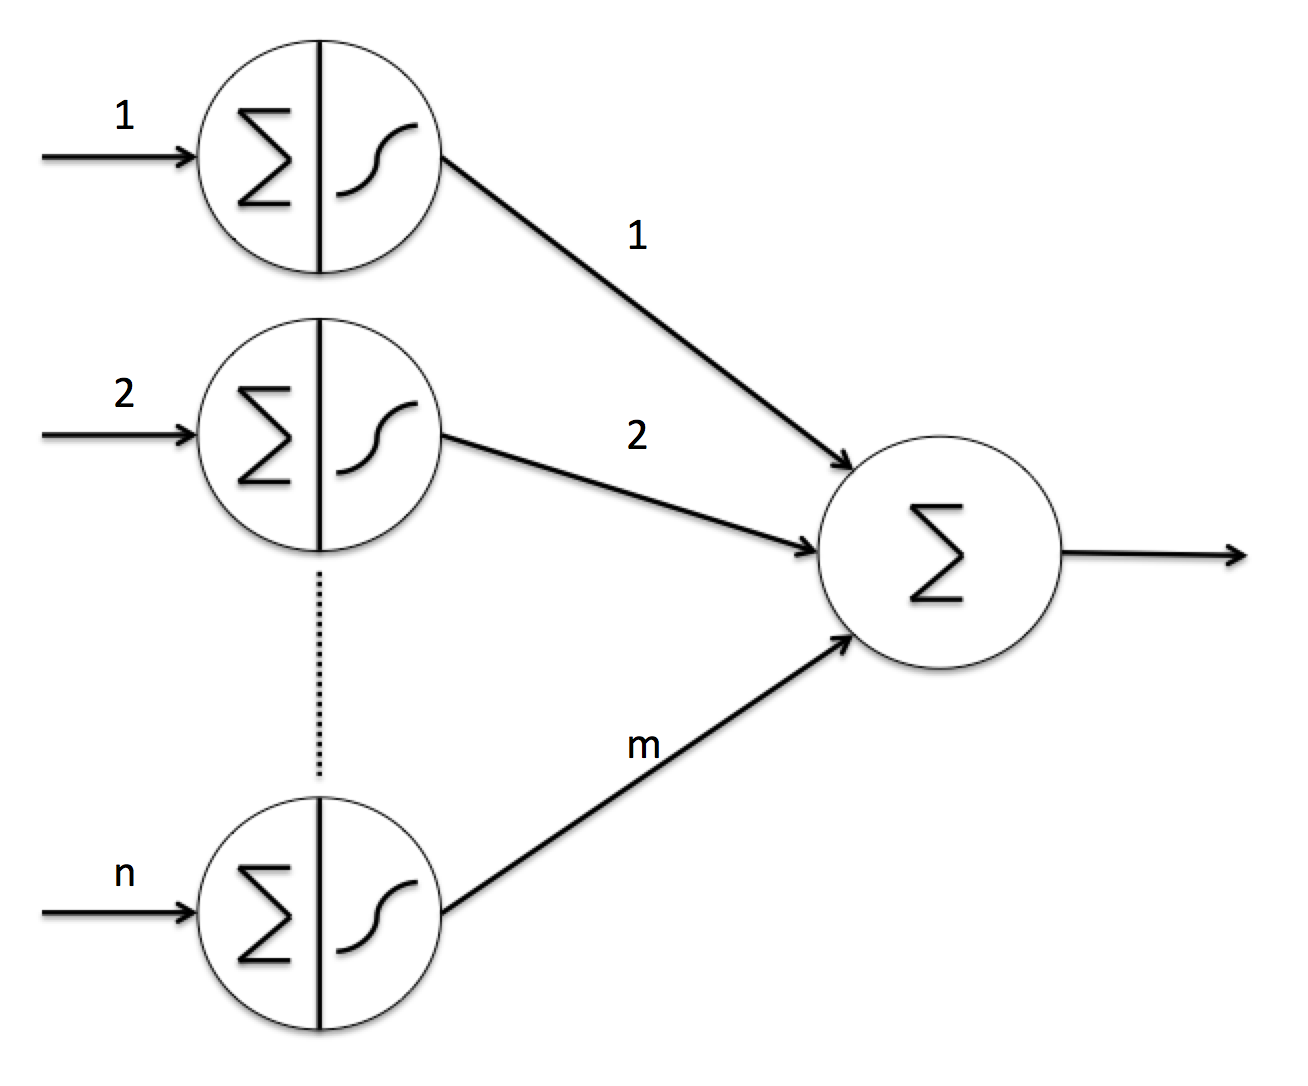
\includegraphics[width=0.8\textwidth]{images/universal_approximator.png}
\end{figure}
\textit{В чем проблема универсального аппроксиматора, исходя из условий теоремы?}

\end{frame}


\begin{frame}{Демонстрация сходимости нейросети с одним скрытым слоем}

\begin{itemize}
	\item операция XOR - 2layer-net-xor.gif
	\item бинарная классификация - 2layer-net-ring.gif
	\item аппроксимация функции sin - 2layer-net-regression-sine.gif
	\item аппроксимация функции abs - 2layer-net-regression-abs.gif\footnote{http://theclevermachine.wordpress.com/2014/09/11/a-gentle-introduction-to-artificial-neural-networks/}
\end{itemize}

\end{frame}


\begin{frame}{Многоснойная нейронная сеть прямого распространения}

\begin{figure}[h!]
  \centering
  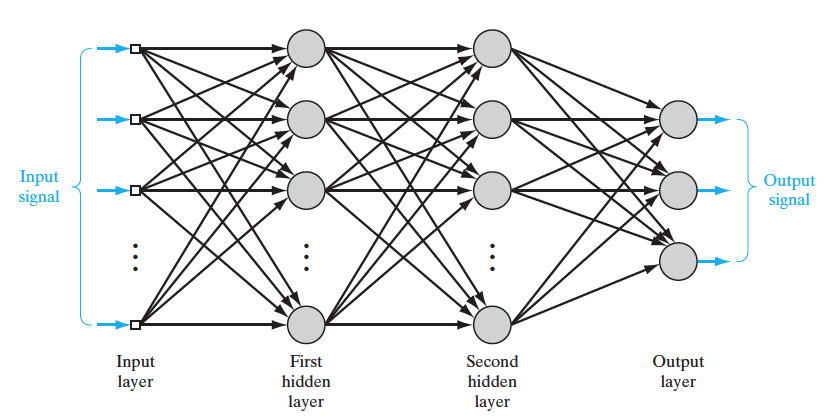
\includegraphics[width=1\textwidth]{images/mlp.png}
  \caption{Архитектура сети с двумя скрытыми слоями\footnote{Neural Networks and Learning Machines (3rd Edition), Simon O. Haykin}}
\end{figure}

\end{frame}

\begin{frame}{Отличие персептрона Румельхарта от персептрона Розенблатта}

\begin{itemize}
	\item Нелинейная функция активации;
	\item один и более скрытых слоев (до работ Хинтона по ограниченной машине Больцмана, на практике не использовали более двух скрытых слоев, а чаще всего один);
	\item сигналы на входе и на выходе не обязательно бинарные;
	\item произвольная архитектура сети (в рамках многослойности);
	\item ошибка сети интерпретирует в смысле некоторой меры, а не как число неправильных образов в режиме обучения.
\end{itemize}

\end{frame}


\begin{frame}{Модифицированная модель нейрона МакКаллока-Питтса}

\begin{figure}[h!]
  \centering
  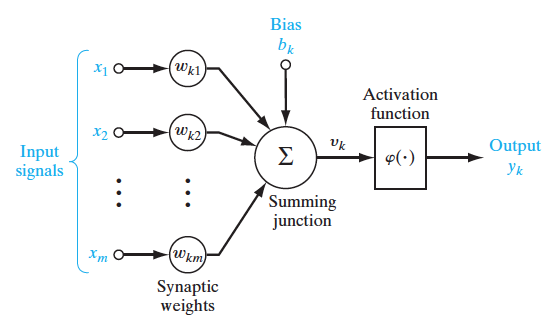
\includegraphics[width=1\textwidth]{images/neuron_mod.png}
  \caption{Схема искусственного нейрона\footnote{Neural Networks and Learning Machines (3rd Edition), Simon O. Haykin}}
\end{figure}

\end{frame}


\begin{frame}{Функция активации}

Задача функции активации - ограничить амплитуду выходного значения нейрона; чаще всего для этого используется одна из сигмоидальных (S-образных) функций:
\begin{itemize}
	\item логистическая функция: $f(z) = \dfrac{1}{1 + e^{-a\cdot z}}, \forall a \in \mathbb{R}$
	\item гиперболический тангенс: $f(z) = \dfrac{e^{a\cdot x} - e^{-a\cdot x}}{e^{a\cdot x} + e^{-a\cdot x}}, \forall a \in \mathbb{R}$
\end{itemize}

\begin{figure}[h!]
  \centering
  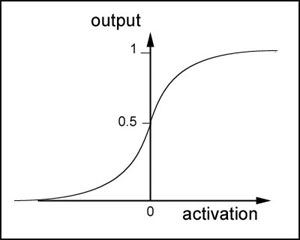
\includegraphics[width=0.5\textwidth]{images/sigmoid.jpg}
  \caption{Логистический сигмоид}
\end{figure}

\end{frame}


\section{Алгоритм обратного распространения ошибки}

\begin{frame}{Backprop, обозначения \#1}

\begin{equation}\label{eq:z}
	z^{(n)}_j = b^{(n)}_j + \sum^{N_{n-1}}_{i=1} w^{(n)}_{ij}x^{(n)}_i = \sum^{N_{n-1}}_{i=0} w^{(n)}_{ij}x^{(n)}_i
\end{equation}
\begin{equation}\label{eq:y}
	y^{(n)}_k = f^{(n)}_k\left(z^{(n)}_k\right)
\end{equation}

\begin{figure}[h!]
  \centering
  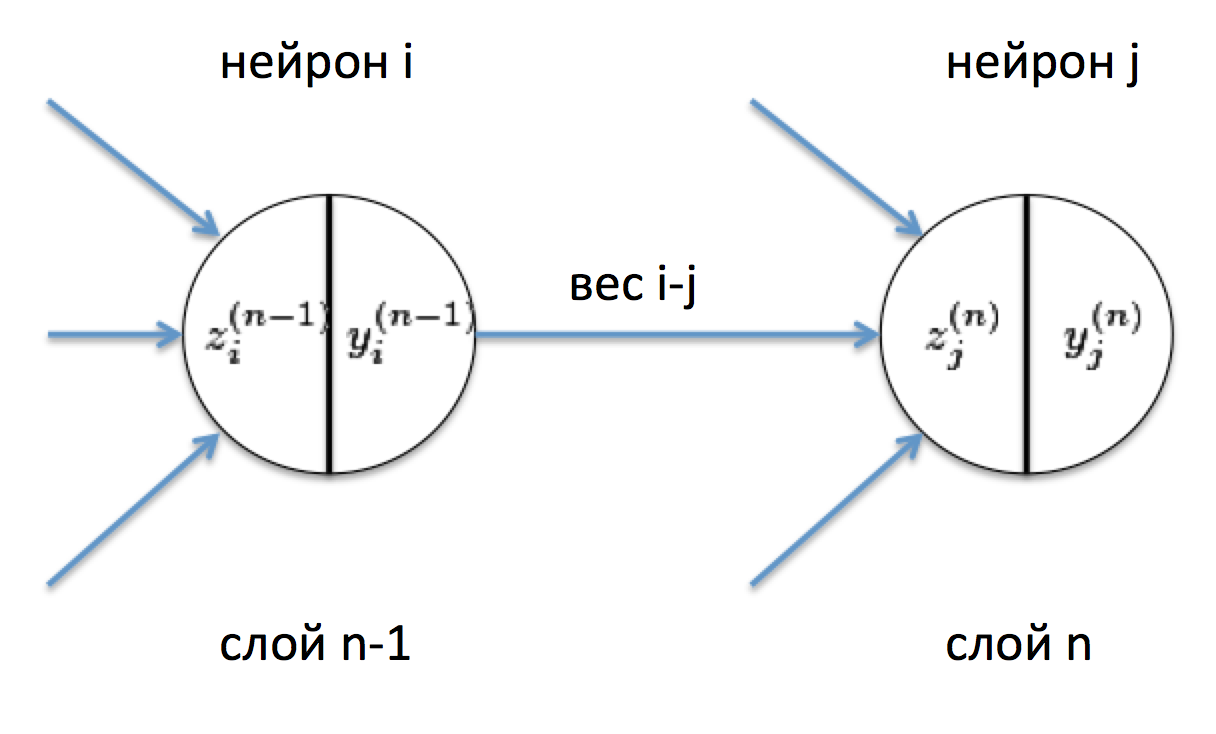
\includegraphics[width=0.9\textwidth]{images/backprop1.png}
  \caption{Схема передачи сигнала между слоями}
\end{figure}

\end{frame}


\begin{frame}{Backprop, обозначения \#2}

Обычное обучение с учителем:
\begin{itemize}
	\item дан набор данных $D = \left\{ \left(x_1, t_1\right), \left(x_2, t_2\right), \ldots, \left(x_{|D|}, t_{|D|}\right) \right\}, x_i \in \mathbb{R}^{N_{\textsc{input}}}, y_i \in \mathbb{R}^{N_{\textsc{output}}}$
	\item необходимо построить такое отображение (нейросеть) $f_{\textsc{network}}: X \rightarrow Y$, которое минимизирует некоторый функционал ошибки $E: \mathbb{R}^{N_{\textsc{output}}} \times \mathbb{R}^{N_{\textsc{output}}} \rightarrow \mathbb{R}$, например
	\begin{itemize}
		\item Евклидово расстояние для задачи регрессии
		\item логарифм функции правдоподобия распределения Бернулли для задачи классификации среди пересекающихся классов
		\item кросс-энтропия для задачи классификации среди \textit{не}пересекающихся классов
	\end{itemize}
\end{itemize}

\end{frame}


\begin{frame}{Градиентный спуск, \#1}

Алгоритм backprop - это модификация классического градиентного спуска. Параметрами модели являются только веса всех нейронов сети:
\begin{equation}\label{eq:delta}
	\delta^{(n)}_{ij} = -\eta \dfrac{\partial E\left( \vec y^{(n)}, \vec t \right)}{\partial w^{(n)}_{ij}}
\end{equation}
\begin{itemize}
	\item $\eta$ - скорость обучения (спуска, learning rate)
	\item $\vec y^{(n)}$ - вектор выходов нейросети (выходы последнего слоя)
	\item $\vec t$ - ожидаемые выходы нейросети для текущего примера
\end{itemize}
\textit{Есть идеи?}

\end{frame}


\begin{frame}[t]{Градиентный спуск, \#2}

\begin{itemize}
	\item $\dfrac{\partial E}{\partial w^{(n)}_{ij}} = \dfrac{\partial E}{\partial z^{(n)}_j} \dfrac{\partial z^{(n)}_j}{\partial w^{(n)}_{ij}}$
	\item \textit{???}
\end{itemize}

\end{frame}


\begin{frame}[t]{Градиентный спуск, \#3}

\begin{itemize}
	\item $\dfrac{\partial E}{\partial w^{(n)}_{ij}} = \dfrac{\partial E}{\partial z^{(n)}_j} \dfrac{\partial z^{(n)}_j}{\partial w^{(n)}_{ij}}$
	\item $\dfrac{\partial z^{(n)}_j}{\partial w^{(n)}_{ij}} = \sum_i \dfrac{\partial w^{(n)}_{ij} x_i^{(n - 1)}}{\partial w^{(n)}_{ij}} = x_i^{(n - 1)}$
\end{itemize}
В итоге получим: 
\begin{equation}\label{eq:de_dw}
	\dfrac{\partial E}{\partial w^{(n)}_{ij}} = x_i^{(n - 1)} \dfrac{\partial E}{\partial z^{(n)}_j}
\end{equation}

\end{frame}


\begin{frame}[t]{Градиентный спуск, выходной слой, \#1}

\begin{itemize}
	\item $\dfrac{\partial E}{\partial w^{(n)}_{ij}} = x_i^{(n - 1)} \dfrac{\partial E}{\partial z^{(n)}_j}$
	\item $E\left(y(z), t\right)$ \textit{???}
\end{itemize}

\end{frame}


\begin{frame}{Градиентный спуск, выходной слой, \#2}

\begin{equation}\label{eq:de_dw_output}
	\dfrac{\partial E}{\partial w^{(n)}_{ij}} = x_i^{(n - 1)} \dfrac{\partial E}{\partial z^{(n)}_j} = x_i^{(n - 1)} \dfrac{\partial E}{\partial y^{(n)}_j} \dfrac{\partial y^{(n)}_j}{\partial z^{(n)}_j}
\end{equation}
Таким образом при условии дифференцируемости целевой функции и функции активации, вычисление градиента любого из весов выходного слоя становится легко решаемой задачей. 

\end{frame}


\begin{frame}[t]{Градиентный спуск, любой скрытый слой, \#1}


\begin{eqnarray*}
	\dfrac{\partial E}{\partial w^{(n)}_{ij}} &=& x^{(n - 1)}_i \dfrac{\partial E}{\partial z^{(n)}_j} \\
	&=& x^{(n - 1)}_i \sum_k \dfrac{\partial E}{\partial z^{(n + 1)}_k} \dfrac{\partial z^{(n + 1)}_k}{\partial z^{(n)}_j} \\
	&=& x^{(n - 1)}_i \sum_k \dfrac{\partial E}{\partial z^{(n + 1)}_k} \dfrac{\partial z^{(n + 1)}_k}{\partial y^{n}_{j}} \dfrac{\partial y^{n}_{j}}{\partial z^{n}_{j}}
\end{eqnarray*}

\begin{itemize}
	\item $\dfrac{\partial z^{(n + 1)}_k}{\partial y^{n}_{j}}$ \textit{???}
\end{itemize}

\end{frame}


\begin{frame}{Градиентный спуск, любой скрытый слой, \#2}

\begin{figure}[h!]
  \centering
  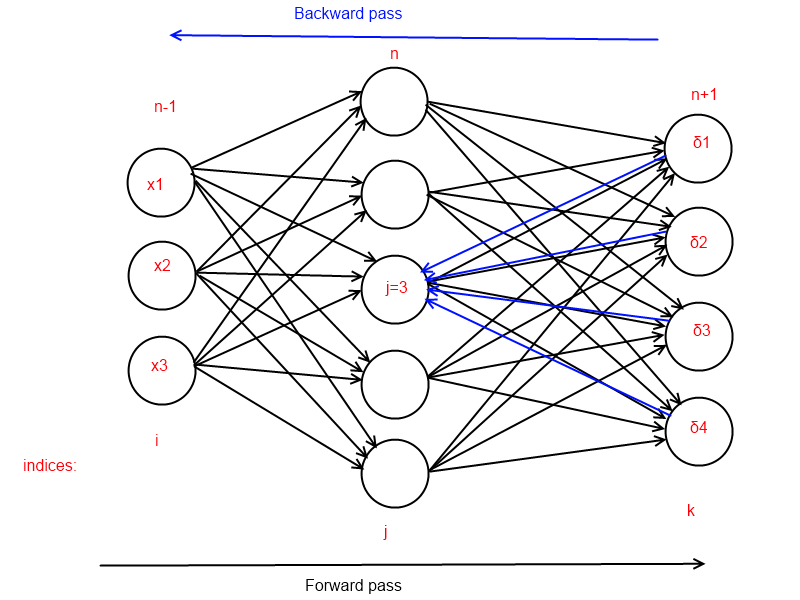
\includegraphics[width=0.9\textwidth]{images/f_b_pass.png}
  \caption{Схема прямого (нелинейного) и обратного (линейного) распространения сигнала в сети}
\end{figure}

\end{frame}


\begin{frame}[t]{Градиентный спуск, любой скрытый слой, \#3}

\begin{eqnarray*}
	\dfrac{\partial E}{\partial w^{(n)}_{ij}} &=& x^{(n - 1)}_i \dfrac{\partial E}{\partial z^{(n)}_j} \\
	&=& x^{(n - 1)}_i \sum_k \dfrac{\partial E}{\partial z^{(n + 1)}_k} \dfrac{\partial z^{(n + 1)}_k}{\partial z^{(n)}_j} \\
	&=& x^{(n - 1)}_i \sum_k \dfrac{\partial E}{\partial z^{(n + 1)}_k} \dfrac{\partial z^{(n + 1)}_k}{\partial y^{n}_{j}} \dfrac{\partial y^{n}_{j}}{\partial z^{n}_{j}}
\end{eqnarray*}

\begin{itemize}
	\item $\dfrac{\partial z^{(n + 1)}_k}{\partial y^{n}_{j}} = \sum_i \dfrac{\partial w^{(n + 1)_{ik}} y^n_i}{\partial y^n_j} = w^{(n + 1)}_{ik}$
\end{itemize}

\end{frame}


\begin{frame}{Градиентный спуск, любой скрытый слой, \#4}

\begin{eqnarray*}
	\dfrac{\partial E}{\partial w^{(n)}_{ij}} &=& x^{(n - 1)}_i \dfrac{\partial E}{\partial z^{(n)}_j} \\
	&=& x^{(n - 1)}_i \sum_k \dfrac{\partial E}{\partial z^{(n + 1)}_k} \dfrac{\partial z^{(n + 1)}_k}{\partial z^{(n)}_j} \\
	&=& x^{(n - 1)}_i \sum_k \dfrac{\partial E}{\partial z^{(n + 1)}_k} \dfrac{\partial z^{(n + 1)}_k}{\partial y^{n}_{j}} \dfrac{\partial y^{n}_{j}}{z^{n}_{j}} \\
	&=& x^{(n - 1)}_i \sum_k w^{(n + 1)}_{ik} \dfrac{\partial E}{\partial z^{(n + 1)}_k}  \dfrac{\partial y^{n}_{j}}{\partial z^{n}_{j}}
\end{eqnarray*}

\end{frame}


\begin{frame}{Некоторые функции стоимости, \#1}

Среднеквадратичная ошибка:
\begin{itemize}
	\item $E = \dfrac{1}{2} \sum_{i \in \textsc{output}} \left( t_i - y_i \right)^2$
	\item $\dfrac{\partial E}{\partial y_i}$ \textit{???}
\end{itemize}

Логарифм правдоподобия Бернулли: 
\begin{itemize}
	\item $E = -\sum_{i \in \textsc{output}} \left( t_i \log y_i + \left( 1 - t_i \right) \log\left( 1 - y_i \right) \right)$
	\item $\dfrac{\partial E}{\partial y_i}$ \textit{???}
\end{itemize}


\end{frame}


\begin{frame}{Некоторые функции стоимости, \#2}

Среднеквадратичная ошибка:
\begin{itemize}
	\item $E = \dfrac{1}{2} \sum_{i \in \textsc{output}} \left( t_i - y_i \right)^2$
	\item $\dfrac{\partial E}{\partial y_i} = y_i - t_i$
\end{itemize}

Логарифм правдоподобия Бернулли: 
\begin{itemize}
	\item $E = -\sum_{i \in \textsc{output}} \left( t_i \log y_i + \left( 1 - t_i \right) \log\left( 1 - y_i \right) \right)$
	\item $\dfrac{\partial E}{\partial y_i} = \dfrac{t_i}{y_i} - \dfrac{1 - t_i}{1 - y_i}$
\end{itemize}


\end{frame}


\begin{frame}{Некоторые функции активации, \#1}

Логистическая функция: 
\begin{itemize}
	\item $f(z) = \dfrac{1}{1 + e^{-a\cdot z}}$
	\item $\dfrac{\partial f}{\partial z}$ \textit{???}
\end{itemize}
Гиперболический тангенс: 
\begin{itemize}
	\item $f(z) = \dfrac{e^{a\cdot z} - e^{-a\cdot z}}{e^{a\cdot z} + e^{-a\cdot z}}$
	\item $\dfrac{\partial f}{\partial z}$ \textit{???}
\end{itemize}

\end{frame}

\begin{frame}{Некоторые функции активации, \#2}

Логистическая функция: 
\begin{itemize}
	\item $f(z) = \dfrac{1}{1 + e^{-a\cdot z}}$
	\item $\dfrac{\partial f}{\partial z} = a \cdot f(z) \cdot \left( 1 - f(x) \right)$
\end{itemize}
Гиперболический тангенс: 
\begin{itemize}
	\item $f(z) = \dfrac{e^{a\cdot z} - e^{-a\cdot z}}{e^{a\cdot z} + e^{-a\cdot z}}$
	\item $\dfrac{\partial f}{\partial z} = a \cdot \left( 1 - f^2(z) \right)$
\end{itemize}

\end{frame}


\begin{frame}{Режимы обучения}

\begin{itemize}
	\item online learning
	\item batch learning
	\item full-batch learning
\end{itemize}

\end{frame}


\begin{frame}{Регуляризация в нейронной сети, \#1}

\textit{Что это и зачем?}

\begin{itemize}
	\item $E_{R} = E\left( \vec y, \vec t \right) + R(W)$
\end{itemize}
Примеры L1 и L2 регуляризации:
\begin{itemize}
	\item $R_{L1}(W) = \sum_{ijn} \left| w_{ij}^{(n)} \right|$
	\item $\dfrac{\partial R_{L1}(W)}{\partial w_{ij}^{(n)}}$ \textit{???}
	\item $R_{L2}(W) = \dfrac{1}{2} \sum_{ijn} \left( w_{ij}^{(n)} \right)^2$
	\item $\dfrac{\partial R_{L2}(W)}{\partial w_{ij}^{(n)}}$ \textit{???}
\end{itemize}

\end{frame}



\begin{frame}{Регуляризация в нейронной сети, \#2}

\begin{itemize}
	\item $E_{R} = E\left( \vec y, \vec t \right) + \lambda \cdot R(W)$
\end{itemize}
Примеры L1 и L2 регуляризации:
\begin{itemize}
	\item $R_{L1}(W) = \sum_{ijn} \left| w_{ij}^{(n)} \right|$
	\item $\dfrac{\partial R_{L1}(W)}{\partial w_{ij}^{(n)}} = \textsc{sign}\left(w_{ij}^{(n)}\right)$
	\item $R_{L2}(W) = \dfrac{1}{2} \sum_{ijn} \left( w_{ij}^{(n)} \right)^2$
	\item $\dfrac{\partial R_{L2}(W)}{\partial w_{ij}^{(n)}} = w_{ij}^{(n)}$
\end{itemize}

\end{frame}


\begin{frame}{Регуляризация в нейронной сети, \#2}

\begin{figure}
        \centering
        \begin{subfigure}[b]{0.5\textwidth}
                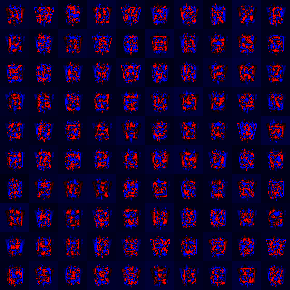
\includegraphics[width=1\textwidth]{images/rbm_colmap_noreg.png}
                \caption{RBM, no reg}                
        \end{subfigure}%        
        \begin{subfigure}[b]{0.5\textwidth}
                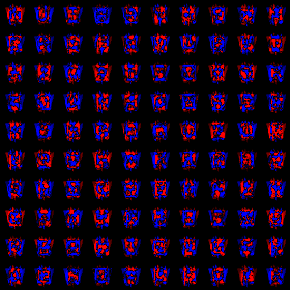
\includegraphics[width=1\textwidth]{images/rbm_colmap_l2.png}
                \caption{RBM, L2 reg}                
        \end{subfigure}       
        \caption{Иллюстрация эффекта регуляризации}
\end{figure}

\end{frame}

\begin{frame}{Регуляризация в нейронной сети, \#3}

\begin{figure}
        \begin{subfigure}[b]{0.5\textwidth}
                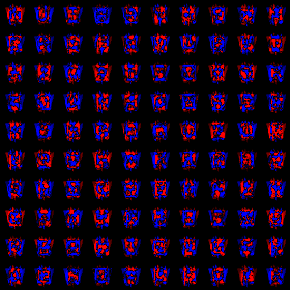
\includegraphics[width=1\textwidth]{images/rbm_colmap_l2.png}
                \caption{RBM, L2 reg}                
        \end{subfigure}%
        \begin{subfigure}[b]{0.5\textwidth}
                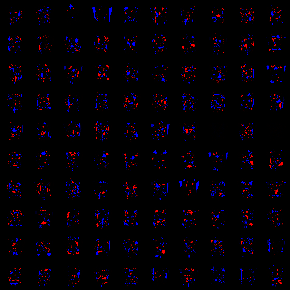
\includegraphics[width=1\textwidth]{images/rbm_colmap_l1.png}
                \caption{RBM, L1 reg}                
        \end{subfigure} 
        \caption{Иллюстрация эффекта регуляризации}
\end{figure}

\end{frame}

\begin{frame}{Критерий остановки}

\begin{figure}[h!]
  \centering
  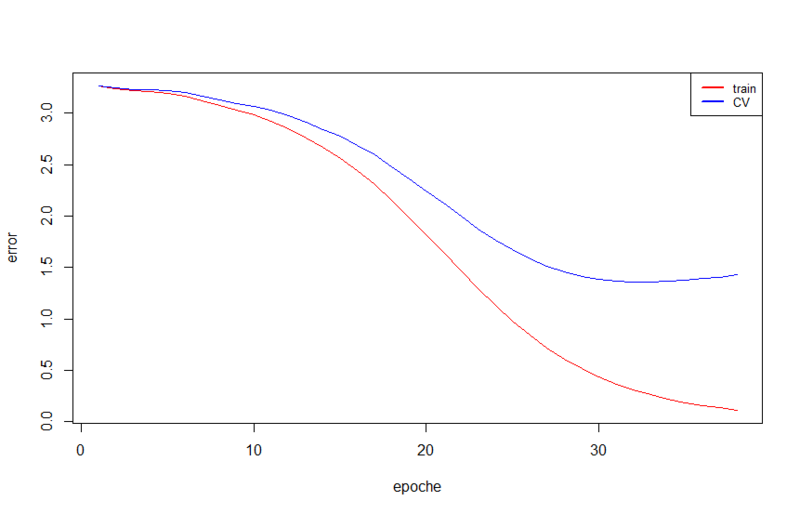
\includegraphics[width=1\textwidth]{images/cv.png}
  \caption{Кроссвалидация}
\end{figure}	
	
\end{frame}


\begin{frame}{Ускорение сходимости}

Добавление момента обучения:
\begin{equation}
\Delta w_{ij}(\tau) = \eta \left( \mu \Delta w_{ij} \left( \tau - 1 \right) + \nabla w_{ij} \right)
\end{equation}

Локальная скорость  обучения:
\begin{equation}
\delta^{(n)}_{ij} = - \eta \cdot r_{ij}^{(n)} \cdot \left( \cdots \right)
\end{equation}
\begin{equation}
r_{ij}^{(n)} = \left\{ { r_{ij}^{(n)} = b + r_{ij}^{(n)}, \nabla w_{ij}^{(n)}(\tau - 1) \cdot \nabla w_{ij}^{(n)}(\tau) > 0 \atop r_{ij}^{(n)} = p \cdot r_{ij}^{(n)} } \right.
\end{equation}
где 
\begin{itemize}
	\item $b$ - аддитивный бонус
	\item $p$ - мультпликативный штраф
	\item $b + p = 1$
	\item естьсмысл добавить верхнюю и нижнюю границы для значения $r_{ij}^{(n)}$
\end{itemize}

\end{frame}


\section{Что дальше?}

\begin{frame}{Планы}

\begin{itemize}
	\item softmax слой в сети прямого распространения
	\item обучение без учителя;
	\item стохастический нейрон и стохастическая нейросеть;
	\item ограниченная машина Больцмана.
	\item глубокие сети
\end{itemize}

\end{frame}


\begin{frame}[plain]
\begin{center}
{\Large Вопросы}
\end{center}
\end{frame}

\end{document}
